%%
% Please see https://bitbucket.org/rivanvx/beamer/wiki/Home for obtaining beamer.
%%
\documentclass[usenames,dvipsnames]{beamer}
\usepackage[utf8]{inputenc}

\setbeamercovered{transparent}
\usetheme{Madrid}
\usefonttheme[onlymath]{serif}
\beamertemplatenavigationsymbolsempty  % remove the navigation bar


% import preamble
%%%%%%%%%%%%%%%%%%%%%%%%%%%%%%%%%%%%%%%%%%%%%%%%%%%%%%%%%%%%%%%%%%%%%%%%%%%%%%%
% begin input file: ./src/preamble.tex
%%%%%%%%%%%%%%%%%%%%%%%%%%%%%%%%%%%%%%%%%%%%%%%%%%%%%%%%%%%%%%%%%%%%%%%%%%%%%%%

%%%
% pre-defined terminologies
\newcommand{\IE}{\textit{i.e.}}
\newcommand{\EG}{\textit{e.g.}}
\newcommand{\WRT}{\textit{w.r.t.}}
\newcommand{\DONUT}{\textit{Donut}}
\newcommand{\DATASETA}{$\mathcal{A}$}
\newcommand{\DATASETB}{$\mathcal{B}$}
\newcommand{\DATASETC}{$\mathcal{C}$}

%%%
% pre-defined content styling macros
\definecolor{emphcolor}{HTML}{007439}
\newcommand{\emphasis}[1]{\textbf{\textcolor{emphcolor}{#1}}}

%%%
% packages and configurations for links
%\usepackage{hyperref}

%%%
% packages for customizing the references
\usepackage{natbib}

%%%
% packages and configurations for `includegraphics`
\usepackage{graphicx}
\usepackage{caption}
\usepackage{subcaption}
\graphicspath{{figures/}}

%%%
% packages and configurations for math equations
\usepackage{array}
\usepackage{amsmath}
\usepackage{amssymb}
\usepackage{bm}
\usepackage{mathtools}

% kill spaces before \left and after \right
\let\originalleft\left
\let\originalright\right
\newcommand{\mleft}{\mathopen{}\mathclose\bgroup\originalleft}
\newcommand{\mright}{\aftergroup\egroup\originalright}

% for common literatures
\newcommand{\grad}{\nabla}
\newcommand{\dd}{\mathrm{d}}
\newcommand{\vv}[1]{\bm{\mathrm{{#1}}}}
\newcommand{\given}{\vert}
\newcommand{\defeq}{\coloneqq}
\DeclareMathOperator*{\argmin}{arg\,min}
\DeclareMathOperator*{\argmax}{arg\,max}
\newcommand{\abs}[1]{\left\lvert{#1}\right\rvert}
\newcommand{\norm}[1]{\left\lVert{#1}\right\rVert}
\newcommand{\numberthis}{\stepcounter{equation}\tag{\theequation}}

% for statistical literatures
\newcommand{\E}{\operatorname{\mathbb{E}}}
\newcommand{\EE}[1]{\operatorname{\mathbb{E}}\mleft[{#1}\mright]}
\newcommand{\EEE}[2]{\operatorname{\mathbb{E}}_{{#1}}\mleft[{#2}\mright]}
\newcommand{\Var}{\operatorname{Var}}
\newcommand{\Varr}[1]{\operatorname{Var}\mleft[{#1}\mright]}
\newcommand{\Varrr}[2]{\operatorname{Var_{{#1}}}\mleft[{#2}\mright]}
\newcommand{\Conv}{\operatorname{Conv}}
\newcommand{\Convv}[2]{\operatorname{Conv}\mleft[{#1},{#2}\mright]}

\newcommand{\KLD}{D_{\text{KL}}}
\newcommand{\KLDD}[2]{\KLD\mleft({#1}\Vert{#2}\mright)}
\newcommand{\Entropy}{H}
\newcommand{\Entropyy}[1]{\Entropy\mleft({#1}\mright)}
\newcommand{\MutualI}{I}
\newcommand{\MutualII}[1]{\MutualI\mleft({#1}\mright)}
\newcommand\independent{\protect\mathpalette{\protect\independenT}{\perp}}
\def\independenT#1#2{\mathrel{\rlap{$#1#2$}\mkern2mu{#1#2}}}

%%%%%%%%%%%%%%%%%%%%%%%%%%%%%%%%%%%%%%%%%%%%%%%%%%%%%%%%%%%%%%%%%%%%%%%%%%%%%%%
% end input file: ./src/preamble.tex
%%%%%%%%%%%%%%%%%%%%%%%%%%%%%%%%%%%%%%%%%%%%%%%%%%%%%%%%%%%%%%%%%%%%%%%%%%%%%%%


% for declaring short slide
\usepackage{etoolbox}
\newtoggle{shortslide}
\togglefalse{shortslide}

% the title
\title{Unsupervised Anomaly Detection via Variational Auto-Encoder for Seasonal KPIs in Web Applications}

\author{
	Haowen Xu\inst{1} \and
	Wenxiao Chen\inst{1} \and
	Nengwen Zhao\inst{1} \and
	Zeyan Li\inst{1} \and
	Jiahao Bu\inst{1} \and
	Zhihan Li\inst{1} \and
	Ying Liu\inst{1} \and
	Youjian Zhao\inst{1} \and
	Dan Pei\inst{1} \and
	Yang Feng\inst{2} \and
	Jie Chen\inst{2} \and
	Zhaogang Wang\inst{2} \and
	Honglin Qiao\inst{2}
}

\institute[]{
	\inst{1} Tsinghua University \and
	\inst{2} Alibaba Group
}

\date{\today}

% At the beginning of each section:
\AtBeginSection[]
{
  \begin{frame}<beamer>{Outline}
    \tableofcontents[currentsection]
  \end{frame}
}

% Let's get started
\begin{document}

\begin{frame}
  \titlepage
\end{frame}

\begin{frame}{Outline}
  \tableofcontents
  % You might wish to add the option [pausesections]
\end{frame}

% main part of the slide
%%%%%%%%%%%%%%%%%%%%%%%%%%%%%%%%%%%%%%%%%%%%%%%%%%%%%%%%%%%%%%%%%%%%%%%%%%%%%%%
% begin input file: ./src/background.tex
%%%%%%%%%%%%%%%%%%%%%%%%%%%%%%%%%%%%%%%%%%%%%%%%%%%%%%%%%%%%%%%%%%%%%%%%%%%%%%%
%%%
\section{Background}

%%
\begin{frame}{Infrastructures for the Information Era is Complicated}
  \begin{figure}
    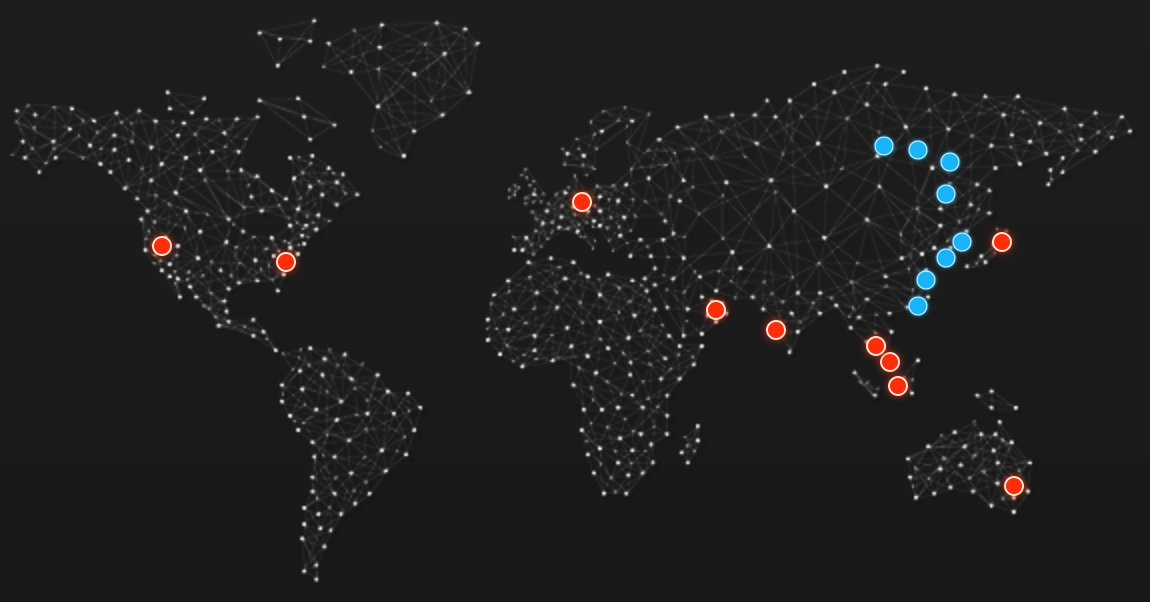
\includegraphics[height=.55\textheight]{alicloud-infra-map}
    \caption{Data centers of AliCloud at 18 global locations.  AliCloud ranks the third in the global public cloud market share. }\label{fig:alicloud-global-infrastructure}
  \end{figure}\vspace{-1em}
  To maintain such huge and complicated system, \emphasis{A}rtificial \emphasis{I}ntelligence for IT \emphasis{Op}eration\emphasis{s} \emphasis{(AIOps)} is greatly demanded.
\end{frame}

%%
\begin{frame}{Anomaly Detection is the First Step for Many AIOps Tasks}
  AIOps consists of many tasks.

  \begin{figure}
  	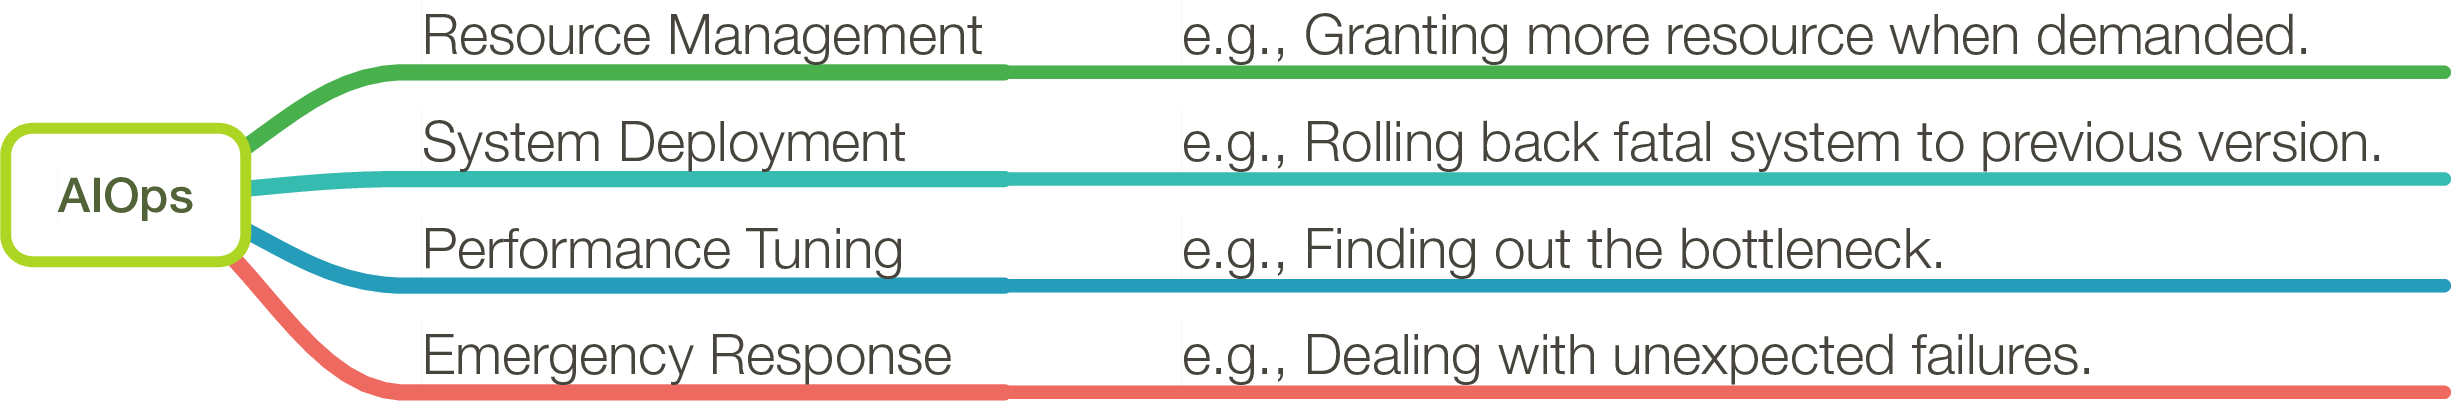
\includegraphics[height=0.21\textheight]{aiops}
  \end{figure}
  
  For most tasks, \emphasis{anomaly detection} is the first step to solve problems.
  In this work, we focus on detecting anomalies on \emphasis{K}ey \emphasis{P}erformance \emphasis{I}ndicators \emphasis{(KPIs)}, which are commonly used as system monitoring.

  \vspace{1em}
  \begin{minipage}{\linewidth}
    \centering
    \begin{figure}
      \begin{subfigure}{0.7\linewidth}
  	    \centering
        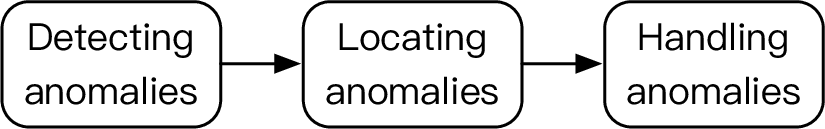
\includegraphics[height=0.14\textheight]{aiops-stages}
        \caption{\footnotesize Anomaly detection is the first step to solve problems.}
      \end{subfigure}\hfill
  	  \begin{subfigure}{0.29\linewidth}
  	    \centering
        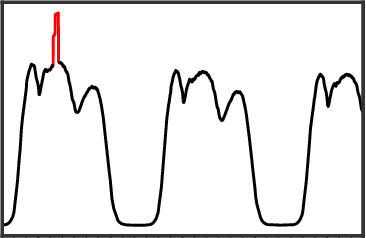
\includegraphics[height=0.14\textheight]{business-kpi}
        \caption{\footnotesize KPI and anomalies.}
      \end{subfigure}
    \end{figure}
  \end{minipage}
\end{frame}

%%
\begin{frame}{Problem Scenario: Anomaly Detection for Seasonal KPIs}
  KPIs are time sequences, yet one of the most fundamental system monitoring indicators.  A failure usually causes more or less anomalies on at least one KPI.  Thus anomaly detection for KPIs are very useful in \emphasis{A}rtificial \emphasis{I}ntelligence for IT \emphasis{Op}eration\emphasis{s} \emphasis{(AIOps)}.\vspace{0.5em}
  
  For web applications, the user activities are usually seasonal, so are the KPIs, including high level KPIs like the trading volumes, and low level KPIs like the CPU consumptions.  We thus focus on \emphasis{anomaly detection for seasonal KPIs in this work}.
  
  \begin{figure}
    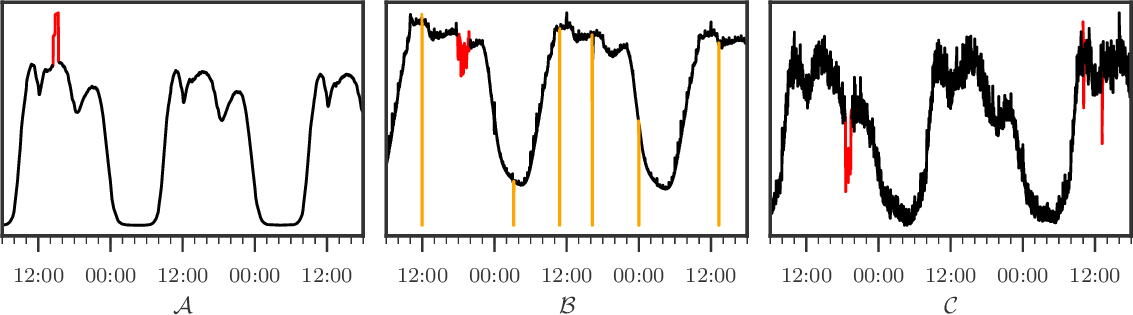
\includegraphics[height=0.36\textheight]{kpi}  
  \end{figure}
\end{frame}

%%
\begin{frame}{Problem Formulation: Detection of ``Abnormal'' Patterns}
  The problem of \emphasis{anomaly detection} can be generally formulated as:
  \begin{block}{Anomaly Detection}
    Detecting whether or not ``abnormal'' patterns occur in the testing data.
  \end{block}
  
  Since KPIs are time sequences, and since in most real cases human operators are willing to see a detection output every time a new observation arrives, the anomaly detection for KPIs can be formulated as:

  \begin{block}{Anomaly Detection for KPIs}
    For each time $t$, given the on-time KPI observation $x_t$ and historical observations $x_{t-W+1}, \dots, x_{t-1}$, determine whether an ``abnormal'' pattern has occurred (denoted by $y_t=1$).
  \end{block}
  
  Detection algorithms are often designed to compute a \emphasis{\textit{real-valued} score} $s(y_t=1)$ (``\emphasis{anomaly score}'' \textit{hereafter}), \EG{}, $p(y_t=1|x_{t-W+1},\dots,x_t)$, leaving the final decision of triggering alerts to the operators.
\end{frame}

%%%
\begin{frame}{Previous Work}
  \vspace{-.5em}
  \begin{itemize}\setlength\itemsep{.2em}
    \item \structure{Anomaly detectors}: \begin{itemize}\small\setlength\itemsep{0em}
        \item \structure{Traditional statistical detectors} are not discriminative enough.  \EG, Holt-Winters, TSD, etc.
        \item \structure{Unsupervised learning based detectors} not good enough in practice.  \EG, one-class SVM, clustering method, K-Means, GMM.
      \end{itemize}
      
    \item \structure{Ensemble learning approaches}: \begin{itemize}\small\setlength\itemsep{0em}
        \item \structure{Supervised ensemble learning} demands too heavily on good labeling quality.  \EG{}, Opprentice~\citep{opprentice}.
        \item \structure{Unsupervised ensemble learning} too sensitive to hyper-parameters.  \EG{}, EGADS~\citep{egads}.
      \end{itemize}
    
    \item \structure{Deep generative models}: \begin{itemize}\small\setlength\itemsep{0em}
        \item \structure{VRNN}~\citep{vi-storn}, uses more advanced model than VAE, but is sensitive to hyper-parameters and extremely slow.  Besides, it lacks \emphasis{dimension reduction}, shown to be essential in our experiments.
      \end{itemize}
  \end{itemize}
  
  \small
  BTW, Opprentice uses \emphasis{14 anomaly detectors} with \emphasis{133 configurations of hyper-parameters}, and is claimed to have better performance than all its components, on datasets very similar to ours.
  We thus use it as a proxy to the traditional detectors in our evaluation.
\end{frame}


%%%%%%%%%%%%%%%%%%%%%%%%%%%%%%%%%%%%%%%%%%%%%%%%%%%%%%%%%%%%%%%%%%%%%%%%%%%%%%%
% end input file: ./src/background.tex
%%%%%%%%%%%%%%%%%%%%%%%%%%%%%%%%%%%%%%%%%%%%%%%%%%%%%%%%%%%%%%%%%%%%%%%%%%%%%%%

%%%%%%%%%%%%%%%%%%%%%%%%%%%%%%%%%%%%%%%%%%%%%%%%%%%%%%%%%%%%%%%%%%%%%%%%%%%%%%%
% begin input file: ./src/architecture.tex
%%%%%%%%%%%%%%%%%%%%%%%%%%%%%%%%%%%%%%%%%%%%%%%%%%%%%%%%%%%%%%%%%%%%%%%%%%%%%%%
\section{Architecture}

%%%
\begin{frame}{The Essential of Stochasticity and Dimension Reduction}
  We carry out some \emphasis{LSTM prediction experiments} at an early stage.
  
  \vspace{-.5em}
  \begin{figure}
    \begin{subfigure}[t]{.49\columnwidth}
      \centering
      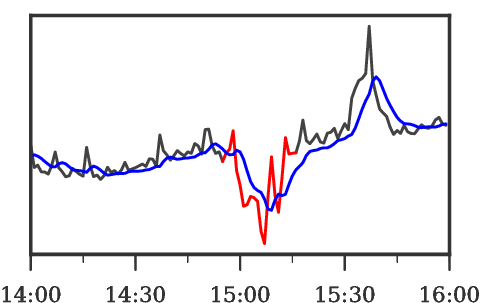
\includegraphics[height=.3\textheight]{kpi_lstm-regression}
    \end{subfigure}\hfill
    \begin{subfigure}[t]{.49\columnwidth}
      \centering
      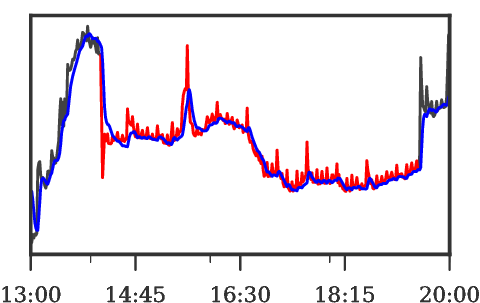
\includegraphics[height=.3\textheight]{kpi_lstm-regression_2}
    \end{subfigure}
  \end{figure}
  \vspace{-.5em}
    
  The LSTM prediction model turns out to be almost a ``\emphasis{lagged copy model}'', hardly valuable for our task.  We thus summarized \emphasis{two essential factors} for anomaly detection via deep neural networks:
  \begin{enumerate}\setlength\itemsep{0em}
    \item \structure{Stochasticity}: The network should be able to capture the stochasticity of ``noises'' on the KPIs internally, to avoid over-fitting.
    \item \structure{Dimension Reduction}: Dimension reduction should be applied, to enforce the network focusing only on the normal patterns of the KPIs.
  \end{enumerate}
  We finally choose the \emphasis{variational auto-encoder (VAE)} to develop our method, according to the above conclusions.
\end{frame}

%%%
\begin{frame}{Background of Variational Auto-Encoder}

  \begin{minipage}[t]{0.25\linewidth}
    \begin{figure}
      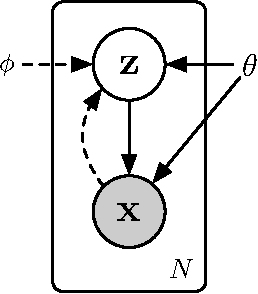
\includegraphics[height=.33\textheight]{variational-auto-encoder}
    \end{figure}
  \end{minipage}\hfill%
  \begin{minipage}[t]{0.74\linewidth}
    VAE models the relationship between two random variables, \emphasis{latent variable $\vv{z}$} and \emphasis{visible variable $\vv{x}$}.  The generative net of VAE consists of:
    \begin{itemize}\setlength\itemsep{0em}
      \item \structure{$\vv{z} \sim p_{\theta}(\vv{z})$}, a chosen prior.
      \item \structure{$\vv{x} \sim p_{\theta}(\vv{x}|\vv{z})$}, derived from a neural network with parameter $\theta$, modeling the data $\vv{x}$.
    \end{itemize}
    The variational net \emphasis{$q_{\phi}(\vv{z}|\vv{x})$} is adopted to approximate the \emphasis{intractable $p_{\theta}(\vv{z}|\vv{x})$}.
    SGVB~\citep{kingma_auto-encoding_2014} is often used to jointly train $q_{\phi}(\vv{z}|\vv{x})$ and $p_{\theta}(\vv{x},\vv{z})$, by maximizing the \emphasis{evidence lower-bound (ELBO)}~\eqref{eqn:elbo}:
  \end{minipage}

  \begin{equation}
    \log p(\vv{x}) \geq \mathcal{L}(\vv{x})
        = \E_{q_{\phi}(\vv{z}|\vv{x})}\Big[\log p_{\theta}(\vv{x}|\vv{z}) + \log p_{\theta}(\vv{z}) - \log q_{\phi}(\vv{z}|\vv{x})\Big]\label{eqn:elbo}
  \end{equation}
  
  Monte Carlo integration can be used to approximate the expectation:
  \[
  \EEE{q_{\phi}(\vv{z}|\vv{x})}{f(\vv{z})} \approx \frac{1}{L} \sum_{l=1}^L f(\vv{z}^{(l)}), \quad \vv{z}^{(l)}\sim q_{\phi}(\vv{z}|\vv{x})
  \]

\end{frame}

%%%
\begin{frame}{Overall Architecture of \DONUT{}}
  \begin{figure}
    \centering
    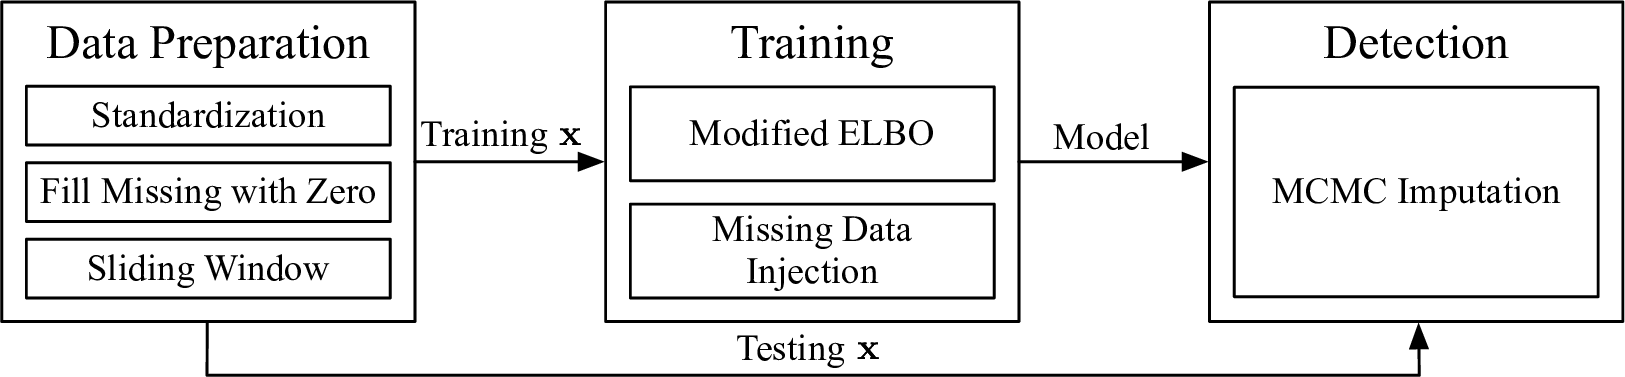
\includegraphics[width=\columnwidth]{architecture}
  \end{figure}
\end{frame}

%%%
\begin{frame}{Data Preparation}
  \begin{itemize}\setlength\itemsep{.2em}
    \item \structure{Fill Missing with Zero}:\\\vspace{.3em}
      \begin{minipage}{0.17\textwidth}
        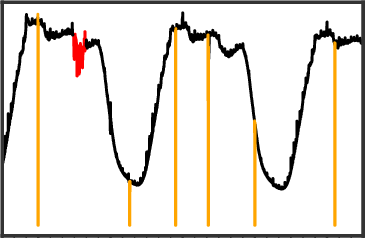
\includegraphics[height=.15\textheight]{fill-missing}  
      \end{minipage}\hfill
      \begin{minipage}{0.73\textwidth}
        \small
        ``Missing'' are special anomalies, \textit{always} known beforehand.
        We fill missing points with zeros (orange points in the left figure), and let our model to handle them afterwards.
      \end{minipage}\vspace{.3em}
    \item \structure{Standardization}: $\hat{x_t} = \mleft(x_t - \mu_x\mright)/\sigma_x$.\\\vspace{.2em}
      {\small $x_t$ are the original KPI values, $\mu_x$ and $\sigma_x$ are the mean and std of $x_t$. \\\vspace{-.2em} We shall use $x_t$ to denote $\hat{x_t}$ and neglect the original values $x_t$ \textit{hereafter}.}
    \item \structure{Sliding Window}:\\\vspace{.3em}
      \begin{minipage}{0.3\textwidth}
        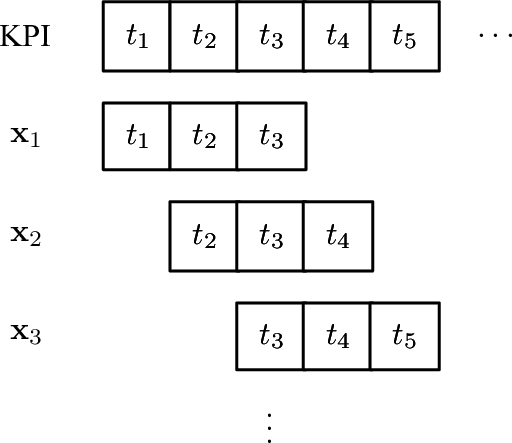
\includegraphics[height=.33\textheight]{sliding-windows}  
      \end{minipage}\hfill
      \begin{minipage}{0.6\textwidth}
        \small
        We split the KPIs into fixed-length \emphasis{sliding windows $\vv{x}_t$}, which are assumed to be \textit{i.i.d.}, and are used as \emphasis{the input $\vv{x}$ of VAE} at every time $t$.
        For simplicity, we shall omit the subscript $t$, using \emphasis{$\vv{x}$} to denote \emphasis{the window of ``current time''}, and \emphasis{$x_1, \dots, x_W$} to denote \emphasis{each point in $\vv{x}$} afterwards.
      \end{minipage}
  \end{itemize}  
\end{frame}

%%%
\begin{frame}{Network Structure}
  \begin{figure}
    \begin{subfigure}[t]{.33\columnwidth}
      \centering
      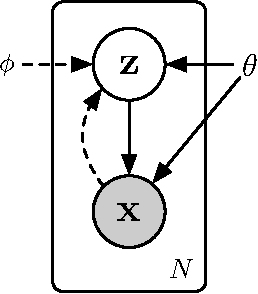
\includegraphics[height=.35\textheight]{variational-auto-encoder}
      \caption{VAE General Structure}
    \end{subfigure}\hfill
    \begin{subfigure}[t]{.33\columnwidth}
      \centering
      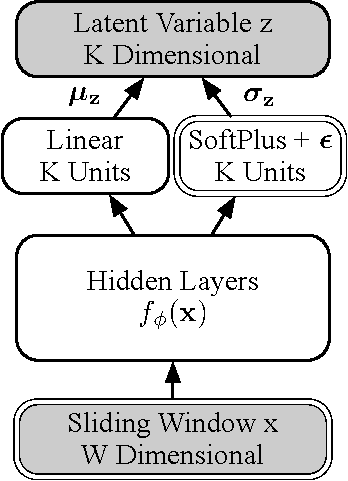
\includegraphics[height=.45\textheight]{variational-net}
      \caption{$q_{\phi}(\vv{z}|\vv{x})$ of \DONUT{}}
    \end{subfigure}\hfill
    \begin{subfigure}[t]{.33\columnwidth}
      \centering
      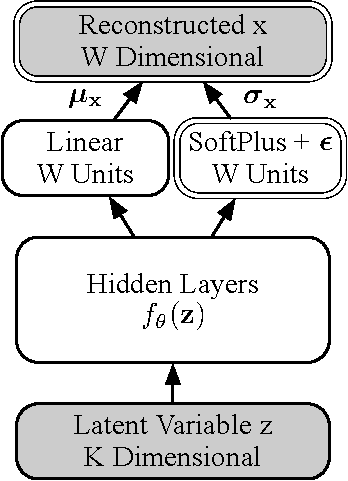
\includegraphics[height=.45\textheight]{generative-net}
      \caption{$p_{\theta}(\vv{x}|\vv{z})$ of \DONUT{}}
    \end{subfigure}
  \end{figure}
  
  \begin{itemize}\setlength\itemsep{.2em}
    \item \structure{Variational net}: $q_{\phi}(\vv{z}|\vv{x})=\mathcal{N}(\vv{\mu_z},\vv{\sigma_z}^2\vv{I})$.
    \item \structure{Generative net}: $p_{\theta}(\vv{z})=\mathcal{N}(\vv{0},\vv{I})$,
      $p_{\theta}(\vv{x}|\vv{z})=\mathcal{N}(\vv{\mu_x},\vv{\sigma_x}^2\vv{I})$.
    \item \structure{SoftPlus Trick}: $\vv{\sigma_z} = \operatorname{SoftPlus}[\vv{W}^{\top}_{\vv{\sigma_z}}f_{\phi}(\vv{x})+\vv{b_{\sigma_z}}] + \vv{\epsilon}$, $\operatorname{SoftPlus}[a] = \;$ $\log [\exp (a) + 1]$.  Similar for $\vv{\sigma_x}$.
  \end{itemize}
\end{frame}

%%%
\begin{frame}{Dealing with Missing and Anomaly: Training}
  \begin{minipage}[t]{.3\linewidth}
    \begin{figure}
      \centering
      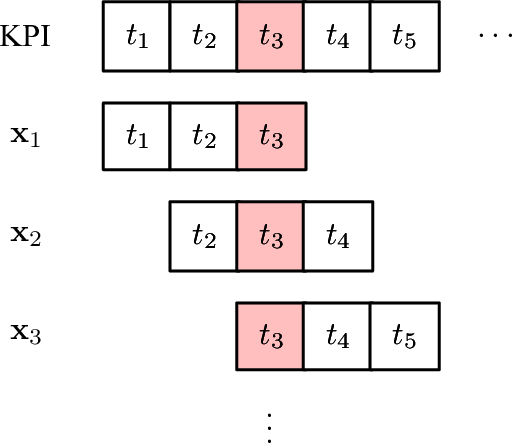
\includegraphics[height=.35\textheight]{sliding-windows-error}
      \caption{The anomaly at $t_3$ shall affect $t_4$ and $t_5$, potentially causing trouble in training and detection.}
    \end{figure}
  \end{minipage}\hfill
  \begin{minipage}[t]{.66\linewidth}
    We developed two techniques to handle such ``historical anomalies'' in training:
    \begin{enumerate}\setlength\itemsep{.2em}
      \item \structure{M-ELBO}: We modify the ELBO~\eqref{eqn:elbo} of VAE into \emphasis{M-ELBO $\widetilde{\mathcal{L}}(\vv{x})$}~\eqref{eqn:m-elbo}. $\alpha_w=1$ indicates $x_w$ being ``normal'', $\alpha_w=0$ otherwise.  $\beta = (\sum_w \alpha_w) / W$.
        We do not exclude ``abnormal'' windows from training data, thus the \emphasis{M-ELBO effectively trains VAE to recover ``normal'' points in $\vv{x}$ even if some ``abnormal'' points exist}.
      \item \structure{Missing Data Injection}: To further amplify the effect of M-ELBO, we randomly set 1\% points to be missing at \emphasis{every epoch}.
    \end{enumerate}
  \end{minipage}
  
  \begin{equation}
    \widetilde{\mathcal{L}}(\vv{x}) = \E_{q_{\phi}(\vv{z}|\vv{x})}\bigg[\sum_{w=1}^W \textcolor{red}{\alpha_w} \log p_{\theta}(x_w|\vv{z}) + \textcolor{red}{\beta} \log p_{\theta}(\vv{z}) - \log q_{\phi}(\vv{z}|\vv{x})\bigg] \label{eqn:m-elbo}
  \end{equation}
\end{frame}

%%%
\begin{frame}{Dealing with Missing and Anomaly: Detection}
  \begin{minipage}[t]{.3\linewidth}
    \begin{figure}
      \centering
      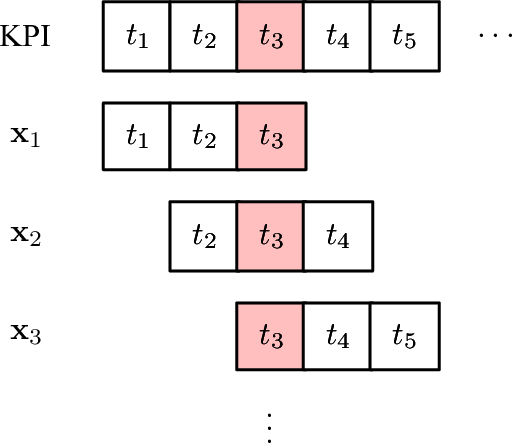
\includegraphics[height=.35\textheight]{sliding-windows-error}
    \end{figure}
  \end{minipage}\hfill
  \begin{minipage}[t]{.66\linewidth}
    In detection, we adopted \structure{MCMC imputation} to impute the already known \emphasis{missing points}, which is proposed by \cite{rezende_stochastic_2014}, using a trained deep generative model to iteratively approach the marginal distribution $p(\vv{x}_{\text{missing}}|\vv{x}_{\text{observed}})$.\vspace{.5em}
    
    The \emphasis{anomalies} other than missing points are to be detected, thus MCMC cannot be applied.  We rely on the effect of \emphasis{dimension reduction} and \emphasis{M-ELBO} to resist such points.
  \end{minipage}
  
  \begin{figure}  
    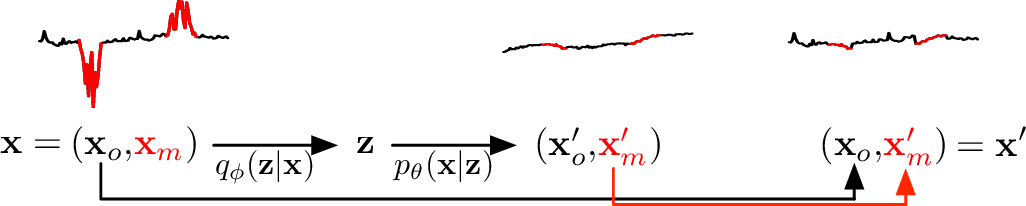
\includegraphics[height=.25\textheight]{mcmc-illustration}
    \caption{Illustration of one iteration in MCMC imputation.}
  \end{figure}
\end{frame}

%%%
\begin{frame}{The Anomaly Score}
  \cite{vae-ad} has already adopted VAE in anomaly detection tasks of other domain\footnote{\cite{vae-ad} uses vanilla VAE, without developing techniques like ours to improve performance.  We shall compare \DONUT{} againt their vanilla VAE in evaluation.}.  They use the \emphasis{reconstruction probability}~\eqref{eqn:reconstruction-probability} of truly \textit{i.i.d.} samples $\vv{x}$ (\EG{}, image pixel vectors) as the anomaly score:
  \begin{equation}\small
    s(y=1) = \EEE{q_{\phi}(\vv{z}|\vv{x})}{\log p_{\theta}(\vv{x}|\vv{z})} \approx
      \frac{1}{L} \sum_{l=1}^L \log p_{\theta}(\vv{x}|\vv{z}^{(l)}), \; \vv{z}^{(l)}\sim q_{\phi}(\vv{z}|\vv{x}) \label{eqn:reconstruction-probability}
  \end{equation}

  Since the KPIs are time sequences, and the operators are willing to see on-time detection outputs each time a new point arrives, we compute the \emphasis{element-wise reconstruction probability}~\eqref{eqn:element-wise-reconstruction-probability} for the last point $x_W$ in $\vv{x}$, as the anomaly score for the time being:
  \begin{equation}\small
    s(y_W=1) = \EEE{q_{\phi}(\vv{z}|\vv{x})}{\log p_{\theta}(x_W|\vv{z})} \approx
      \frac{1}{L} \sum_{l=1}^L \log p_{\theta}(x_W|\vv{z}^{(l)}), \; \vv{z}^{(l)}\sim q_{\phi}(\vv{z}|\vv{x}) \label{eqn:element-wise-reconstruction-probability}
  \end{equation}
  
\end{frame}


%%%%%%%%%%%%%%%%%%%%%%%%%%%%%%%%%%%%%%%%%%%%%%%%%%%%%%%%%%%%%%%%%%%%%%%%%%%%%%%
% end input file: ./src/architecture.tex
%%%%%%%%%%%%%%%%%%%%%%%%%%%%%%%%%%%%%%%%%%%%%%%%%%%%%%%%%%%%%%%%%%%%%%%%%%%%%%%

%%%%%%%%%%%%%%%%%%%%%%%%%%%%%%%%%%%%%%%%%%%%%%%%%%%%%%%%%%%%%%%%%%%%%%%%%%%%%%%
% begin input file: ./src/evaluation.tex
%%%%%%%%%%%%%%%%%%%%%%%%%%%%%%%%%%%%%%%%%%%%%%%%%%%%%%%%%%%%%%%%%%%%%%%%%%%%%%%
\section{Evaluation}

%%%
\begin{frame}{Datasets for Evaluation}
  \vspace{-1em}
  \begin{figure}
    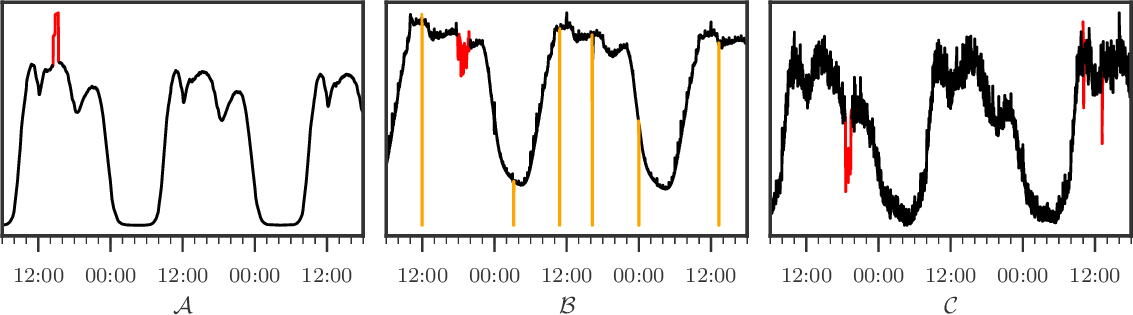
\includegraphics[height=.3\textheight]{kpi}  
  \end{figure}
  \vspace{-1.5em}
  \begin{table}[htbp]
    \footnotesize
    \centering
    \begin{tabular}{
              |p{.25\textwidth}
              |p{.15\textwidth}
              |p{.15\textwidth}
              |p{.15\textwidth}
              |
      }
      \hline
      DataSet & \DATASETA{} & \DATASETB{} & \DATASETC{}  \\
      \hline
      Total points & 296460 & 317522 & 285120  \\
      Missing points & 1222/0.41\% & 1117/0.35\% & 304/0.11\%  \\
      Anomaly points & 1213/0.41\% & 1883/0.59\% & 4394/1.54\%  \\
      Total windows & 296341 & 317403 & 285001  \\
      Abnormal windows & 20460/6.90\% & 20747/6.54\%  & 17288/6.07\%  \\
      \hline
    \end{tabular}
  \end{table}
  
  \small
  We obtain 18 well-maintained KPIs from Alibaba Group, and choose 3 of them, denoted as \DATASETA{}, \DATASETB{} and \DATASETC{}, with relatively small, medium and large noises among the 18 datasets, so we can \emphasis{evaluate \DONUT{} for noises at different levels}.
\end{frame}

%%%
\begin{frame}{Performance Metrics}
  \small
  A \emphasis{threshold} is needed to turn anomaly scores into \emphasis{alerts}.
  In practice, the total number of alerts are often controlled by adjusting the thresholds, we thus report the following metrics, as evaluation of the overall performance of a model:
  \begin{enumerate}\small\setlength\itemsep{0em}
    \item \structure{AUC}: The \emphasis{average precision over recalls}, given all possible thresholds.
    \item \structure{Best F-score}: The \emphasis{largest F-score} (F-score is the harmonic mean of precision and recall), given all possible thresholds.
  \end{enumerate}

  \small
  In real applications, it is acceptable for an algorithm to \emphasis{trigger an alert for any point in a contiguous anomaly segment}, if the delay is not too long.  We thus modify the two metrics to reflect such preference:
  
  \vspace{1em}
  \begin{minipage}{0.54\textwidth}
    \begin{figure}
	  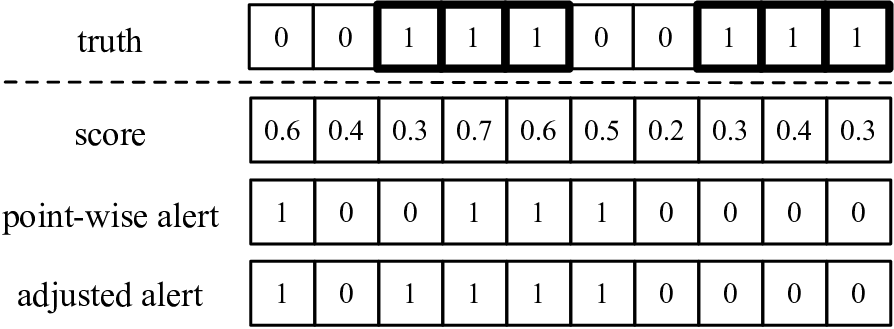
\includegraphics[height=.26\textheight]{metric-illustration}
    \end{figure}
  \end{minipage}\hfill
  \begin{minipage}{0.43\textwidth}
   \structure{1st row}: ground truth; \structure{2nd row}: detection scores; \structure{3rd row}: point-wise alerts outputs with a threshold of 0.5; \structure{4th row}: adjusted point-wise alerts.  We use the adjusted alerts to compute the metrics.
  \end{minipage}
\end{frame}

%%%
\begin{frame}{Experiment Setup}
  \vspace{-.5em}

  \structure{Major hyper-parameters\footnote{The rest can be found in the paper.} of \DONUT{}}
  \begin{table}[htbp]
    \footnotesize
    \centering
    \begin{tabular}{
            |p{.12\textwidth}
            |p{.25\textwidth}
            |p{.48\textwidth}
            |
      }
      \hline
      Parameter & Choice & Description  \\
      \hline
      $W$ & $120$ & Window size of $\vv{x}$. \\
      $K$ & $8$ (\DATASETA{}), $3$ (\DATASETB{} and \DATASETC{}) & Number of $\vv{z}$ dimensions. \\
      $f_{\phi}(\vv{x})$ & $2$ Layers of $100$ ReLU & Hidden layers of $q_{\phi}(\vv{z}|\vv{x})$. \\
      $f_{\theta}(\vv{z})$ & $2$ Layers of $100$ ReLU & Hidden layers of $p_{\theta}(\vv{x}|\vv{z})$. \\
      $\epsilon$ & $10^{-4}$ & Minimum output value for the std layers. \\
      $\lambda$ & $0.01$ & Missing data injection ratio. \\
      $M$ & $10$ & MCMC iteration count. \\
      $L$ & $1024$ & Monte Carlo integration sampling number. \\
      \hline
    \end{tabular}
  \end{table}
  
  \structure{Algorithms for comparison}\vspace{.2em}
  \begin{enumerate}\small\setlength\itemsep{.2em}
    \item \structure{Opprentice}~\citep{opprentice}: supervised ensemble learning, based on 14 traditional detectors with 133 hyper-parameter configurations.
    \item \structure{VAE Baseline}: vanilla VAE for anomaly detection on \textit{i.i.d.} samples~\citep{vae-ad}.  Hyper-parameters are chosen to be identical with \DONUT{}.
    \item \structure{\DONUT{}-Prior}: identical with \DONUT{}, expect for using $\EEE{p_{\theta}(\vv{z})}{\log p_{\theta}(\vv{x}|\vv{z})}$ instead of the reconstruction probability $\EEE{q_{\phi}(\vv{z}|\vv{x})}{\log p_{\theta}(\vv{x}|\vv{z})}$.
  \end{enumerate}
  \vspace{.5em}
\end{frame}

%%%
\begin{frame}{Overall Performance}
  \begin{figure}
    \centering
    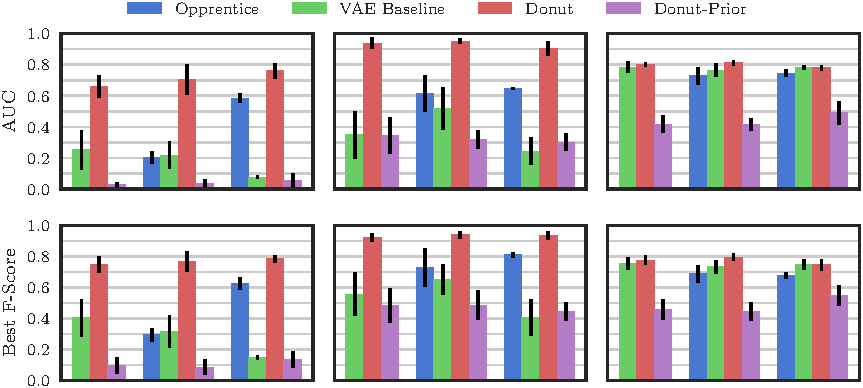
\includegraphics[height=11.7em]{overall_perf}\\\vspace{.6em}
    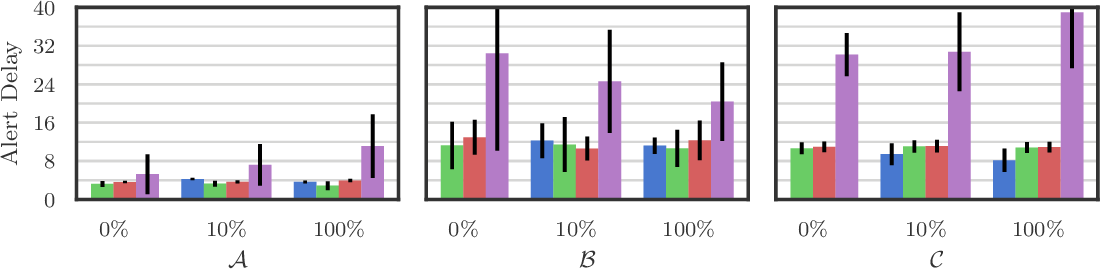
\includegraphics[height=6.35em]{delay_perf}
  \end{figure}
\end{frame}

%%%
\begin{frame}{Effects of \DONUT{} Techniques}
  \begin{figure}
    \centering
    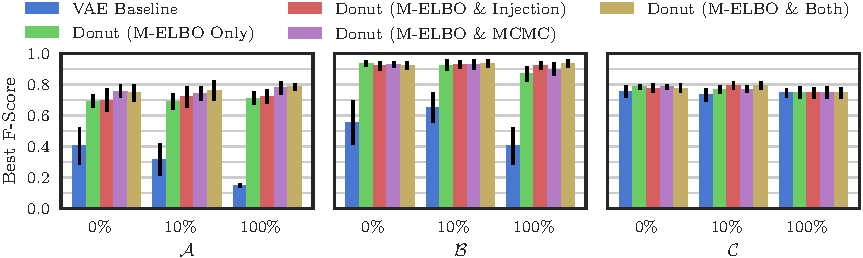
\includegraphics[height=.39\textheight]{tricks_perf}
    \caption{
		Best F-score of (1) VAE Baseline, (2) \DONUT{} with M-ELBO, (3) M-ELBO + missing data injection, (4) M-ELBO + MCMC, and (5) M-ELBO + both MCMC and injection.
    }
  \end{figure}\vspace{-1em}
  
  The \emphasis{M-ELBO} alone contributes most of the improvement over VAE Baseline, while the \emphasis{missing data injection} and the \emphasis{MCMC imputation} can further benefit the performance.
\end{frame}

%%%
\begin{frame}{Impact of Z Dimension Number K}
  \begin{figure}
    \centering
    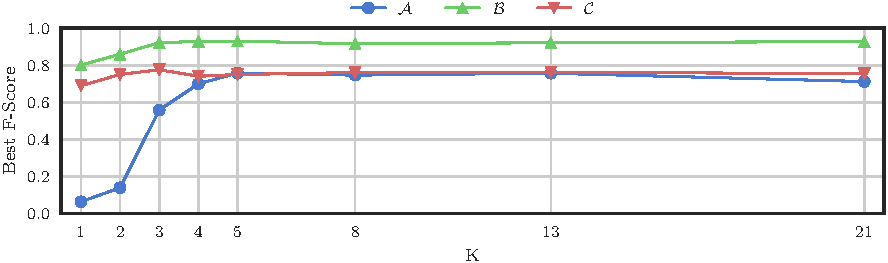
\includegraphics[height=.37\textheight]{z_dim_fscore_000}
	\caption{
      The best F-score of unsupervised \DONUT{} with different $K$ on testing set.
    }
  \end{figure}
  \vspace{-1em}

  \begin{itemize}\setlength\itemsep{.2em}
    \item The essential of \emphasis{Dimension reduction}: $W$ (the dimension of $\vv{x}$) is 120, while the best $K$ (the dimension of $\vv{z}$) is no larger than 10.
    \item It should be quite easy to empirically choose $K$.
      \begin{enumerate}\setlength\itemsep{0em}
        \item The best performance could be achieved with fairly small $K$.
        \item The performance does not drop too heavily for $K$ up to 21.
      \end{enumerate}
    \item Smoother KPIs seem to demand larger $K$.
  \end{itemize}
\end{frame}

%%%%%%%%%%%%%%%%%%%%%%%%%%%%%%%%%%%%%%%%%%%%%%%%%%%%%%%%%%%%%%%%%%%%%%%%%%%%%%%
% end input file: ./src/evaluation.tex
%%%%%%%%%%%%%%%%%%%%%%%%%%%%%%%%%%%%%%%%%%%%%%%%%%%%%%%%%%%%%%%%%%%%%%%%%%%%%%%

%%%%%%%%%%%%%%%%%%%%%%%%%%%%%%%%%%%%%%%%%%%%%%%%%%%%%%%%%%%%%%%%%%%%%%%%%%%%%%%
% begin input file: ./src/analysis.tex
%%%%%%%%%%%%%%%%%%%%%%%%%%%%%%%%%%%%%%%%%%%%%%%%%%%%%%%%%%%%%%%%%%%%%%%%%%%%%%%
\section{Analysis}

%%%
\begin{frame}{Reconstruction Probability isn't a Well-Defined Probability}
  The \structure{reconstruction probability}, defined by:
  \[
  \EEE{q_{\phi}(\vv{z}|\vv{x})}{\log p_{\theta}(\vv{x}|\vv{z})}
		= \int q_{\phi}(\vv{z}|\vv{x}) \log p_{\theta}(\vv{x}|\vv{z}) \dd\vv{z}
  \]
  \emphasis{is quite absurd}, since we can easily notice that, the following equation is not well-defined under the probability framework:
  \[
  \EEE{q_{\phi}(\vv{z}|\vv{x})}{p_{\theta}(\vv{x}|\vv{z})}
		= \int q_{\phi}(\vv{z}|\vv{x}) \, p_{\theta}(\vv{x}|\vv{z}) \dd\vv{z}
  \]
  \cite{vae-ad} just uses the reconstruction probability as the anomaly score, without solid theoretical explanation.  Meanwhile, \structure{the prior counterpart, \IE{}, $\EEE{p_{\theta}(\vv{z})}{\log p(\vv{x}|\vv{z})}$}, which is more reasonable under the probability framework, since $p(\vv{x}) = \EEE{p_{\theta}(\vv{z})}{p(\vv{x}|\vv{z})}$ is well-defined, but actually shows \emphasis{much worse performance} in evaluation.
\end{frame}

%%%
\begin{frame}{The Time Gradient}
  \begin{minipage}{0.45\textwidth}
    \begin{figure}
      \centering
      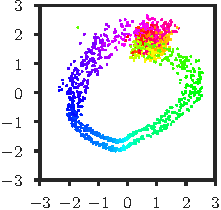
\includegraphics[height=.4\textheight]{z2_latent_space_normal}
      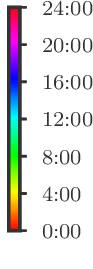
\includegraphics[height=.4\textheight]{z2_latent_space_bar}
      \caption{
        The $\vv{z}$ layout of dataset \DATASETB{}.
        Figure is plotted by sampling $\vv{z}$ from $q_{\phi}(\vv{z}|\vv{x})$, corresponding to normal $\vv{x}$ randomly chosen from the testing set.
        $K$ is chosen as 2, so the x- and y-axis are the two dimensions of $\vv{z}$ samples.
        The color of a $\vv{z}$ sample denotes its time of the day.
      }
    \end{figure}
  \end{minipage}\hfill
  \begin{minipage}{0.52\textwidth}
    \small
    \begin{itemize}\setlength\itemsep{.2em}
      \item \structure{Time gradient}: $q_{\phi}(\vv{z}|\vv{x})$ are organized in smooth transition: $\vv{x}$ at contiguous time are mapped to nearby $q_{\phi}(\vv{z}|\vv{x})$.
      \item \structure{Contiguous $\vv{x}$ are highly similar in the KPIs of our interest}, since they are smooth in general.
      \item \structure{Transition of $q_{\phi}(\vv{z}|\vv{x})$ in the shape of $\vv{x}$ rather than time is the cause of time gradient}, since \DONUT{} consumes no time information.
      \item \structure{\DONUT{} encodes the ``shape'' or ``normal patterns'' of $\vv{x}$ by $\vv{z}$}, as shown by the time gradient.
      \item \structure{The time gradient can benefit generalization}.
    \end{itemize}
  \end{minipage}
\end{frame}

%%%
\begin{frame}{Layouts of $\vv{z}$ for All Three Datasets when $K=3$}
  \begin{figure}
    \centering
    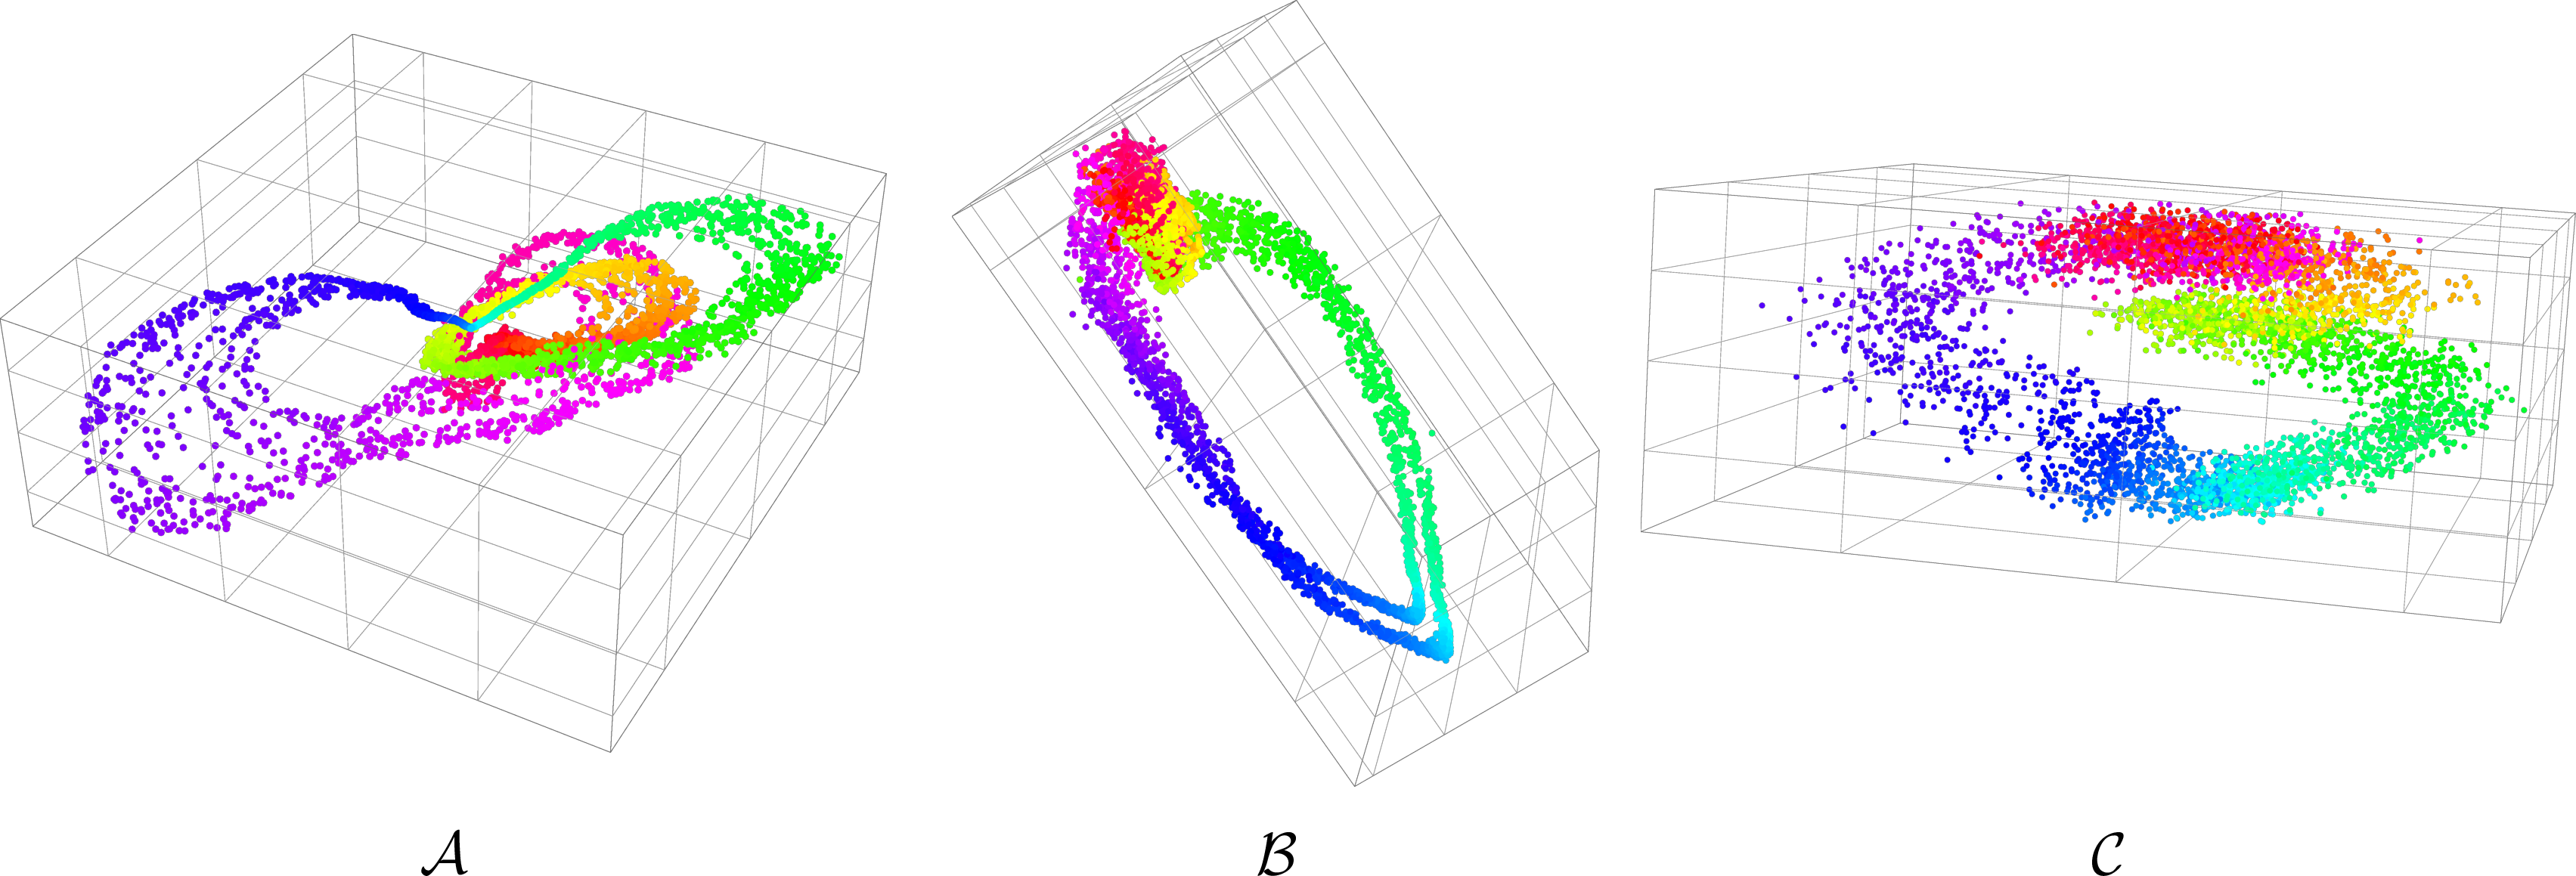
\includegraphics[width=\textwidth]{z3_latent_space}
  \end{figure}
\end{frame}

%%%
\begin{frame}{The KDE Interpretation}
  \begin{figure}
    \centering
    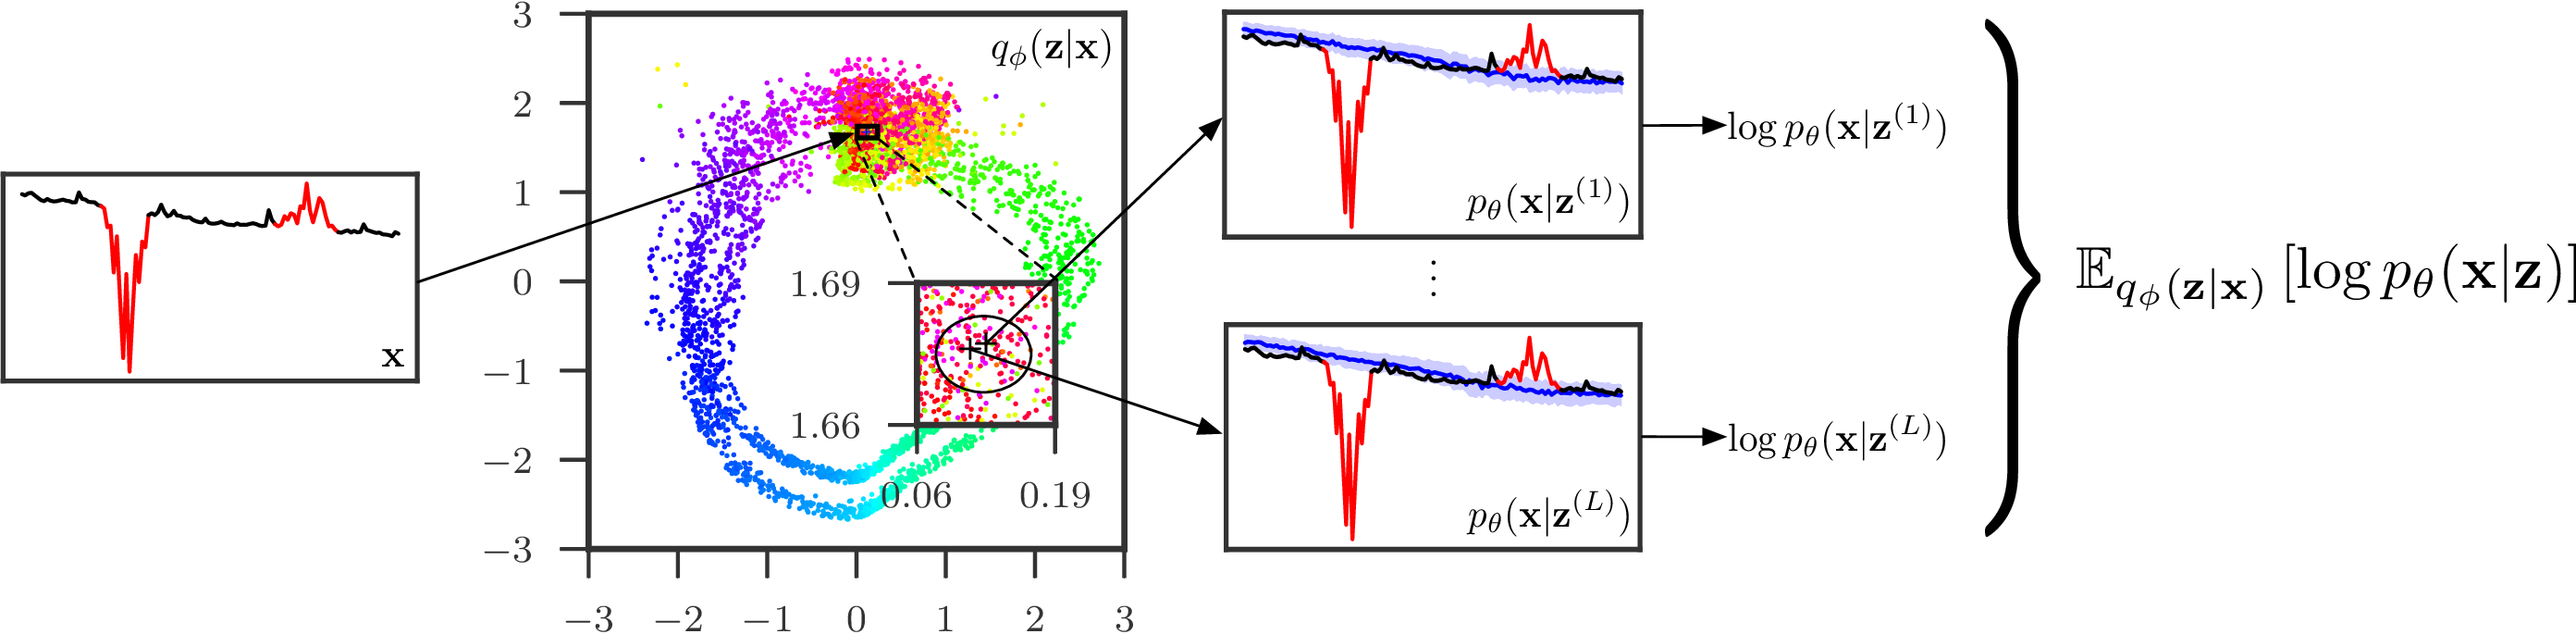
\includegraphics[width=\textwidth]{kde_interpretation}
    \vspace{.5em}
    \caption{
      Illustration of the KDE interpretation.
      \emphasis{For a given $\vv{x}$ potentially with anomalies, \DONUT{} tries to recognize what normal pattern it follows, encoded as $q_{\phi}(\vv{z}|\vv{x})$}.
      The black ellipse in the middle figure denotes the 3-$\vv{\sigma_z}$ region of $q_{\phi}(\vv{z}|\vv{x})$.
      \emphasis{$L$ samples of $\vv{z}$ are then taken from $q_{\phi}(\vv{z}|\vv{x})$}, denoted as the crosses in the middle figure.
      \emphasis{Each $\vv{z}$ is associated with a density estimator kernel $\log p_{\theta}(\vv{x}|\vv{z})$}.
      The blue curves in the right two figures are $\vv{\mu_x}$ of each kernel, while the surrounding stripes are $\vv{\sigma_x}$.
      Finally, the \emphasis{values of $\log p_{\theta}(\vv{x}|\vv{z})$ are computed from each kernel, and further averaged together as the reconstruction probability}.
    }
    \label{fig:kde-interpretation}
  \end{figure}
\end{frame}

%%%
\begin{frame}{Find Good Posteriors for Abnormal $\vv{x}$}
  All the following techniques work by improving the ability of \DONUT{} to find ``good'' posteriors\footnote{``good'' implies beneficial for the anomaly detection task.} for abnormal $\vv{x}$:

  \begin{itemize}\setlength\itemsep{.2em}
    \item \structure{Dimension Reduction}: Force \DONUT{} to focus only on normal patterns.
    \item \structure{M-ELBO}: Explicitly trains \DONUT{} to recover normal points even when abnormal points exist in $\vv{x}$.
    \item \structure{Missing Data Injection}: Amplifies the effect of \textit{M-ELBO}.
    \item \structure{MCMC Imputation}: Alleviate the biases brought by missing points, helping \DONUT{} to find good posteriors.
  \end{itemize}
\end{frame}

%%%
\begin{frame}{Visualization of MCMC Imputation}
  \begin{figure}
    \centering
    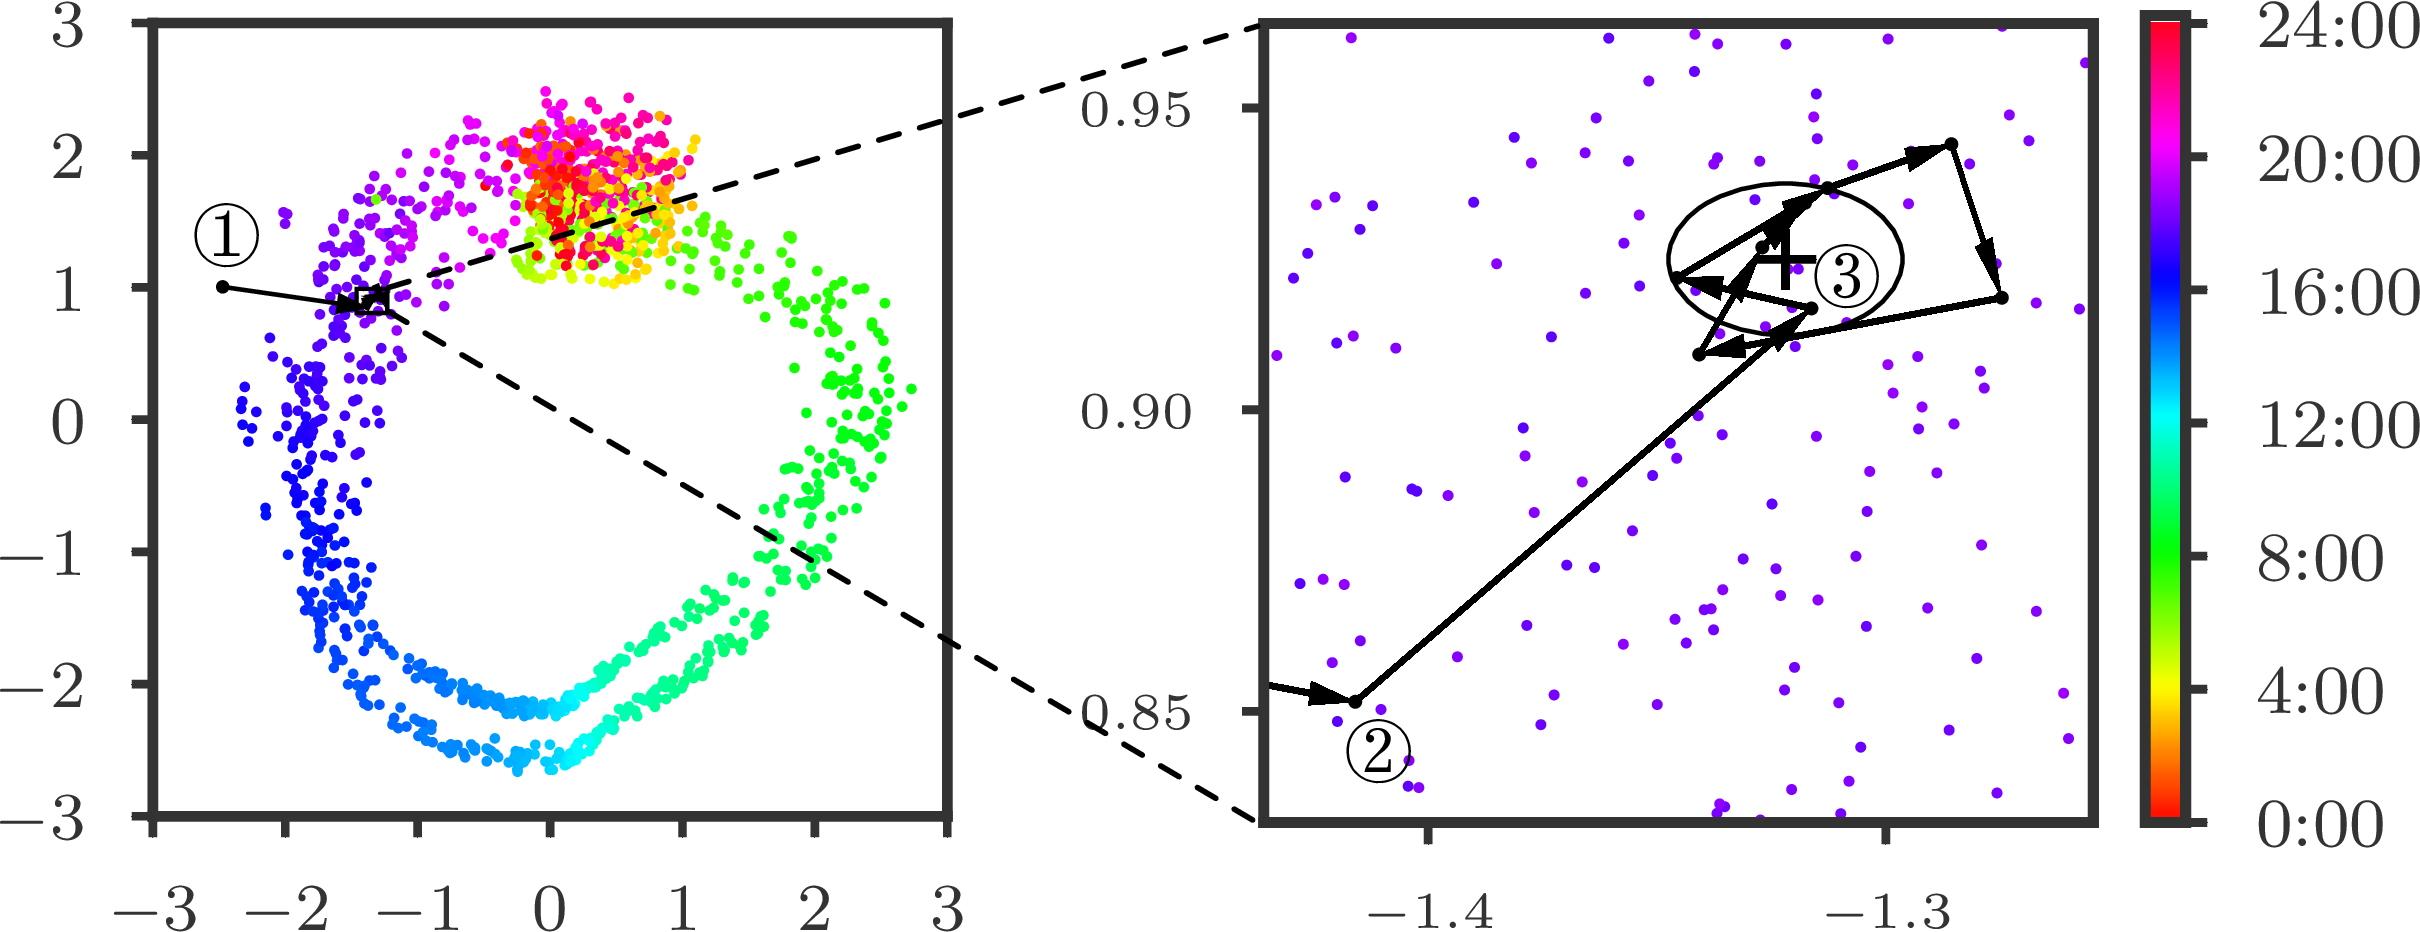
\includegraphics[height=.5\textheight]{mcmc_z_trace}
	\caption{
		MCMC visualization.
		A normal $\vv{x}$ is chosen, whose posterior $q_{\phi}(\vv{z}|\vv{x})$ is plotted at right: the cross denotes $\vv{\mu_z}$ and the ellipse denotes its 3-$\vv{\sigma_z}$ region.
		We randomly set 15\% $\vv{x}$ points as missing, to obtain the abnormal $\vv{x}'$.
		We run MCMC over $\vv{x}'$ with 10 iterations.
		At first, the $\vv{z}$ sample is far from $q_{\phi}(\vv{z}|\vv{x})$.
		After that, $\vv{z}$ samples quickly approach $q_{\phi}(\vv{z}|\vv{x})$, and begin to move around $q_{\phi}(\vv{z}|\vv{x})$ after only 3 iterations.
	}
  \end{figure}
\end{frame}

%%%
\begin{frame}{Revisit of the Causes of Time Gradient}
  \begin{figure}
    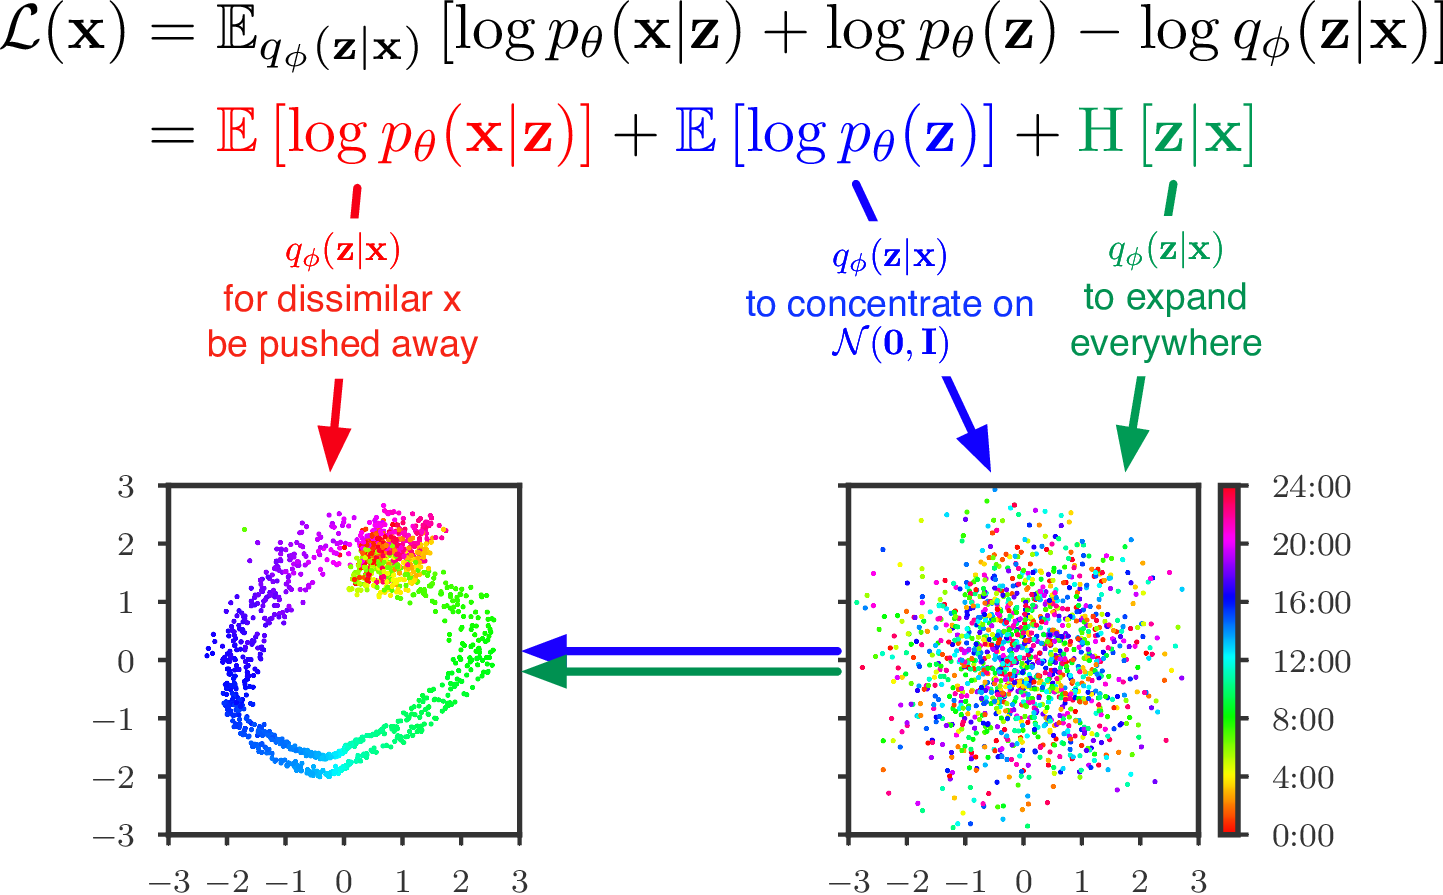
\includegraphics[height=.63\textheight]{time-gradient-causes}
    \caption{
      Causes of the time gradient.
      Surprisingly, we find no term in ELBO directly pulling $q_{\phi}(\vv{z}|\vv{x})$ for similar $\vv{x}$ together.
      The time gradient is likely to be caused mainly by \emphasis{expansion} ($\Entropyy{\vv{z}|\vv{x}}$), \emphasis{squeezing} ($\EE{\log p_{\theta}(\vv{z})}$), \emphasis{pushing} ($\EE{\log p_{\theta}(\vv{x}|\vv{z})}$), and the \emphasis{training dynamics} (random initialization and SGVB).  
    }
  \end{figure}
\end{frame}

%%%
\begin{frame}{Sub-Optimal Equilibrium}
  The training dynamics may cause sub-optimal equilibrium.  Having larger $K$ (number of $\vv{z}$ dimensions) might help to avoid such problems.

  \begin{figure}
    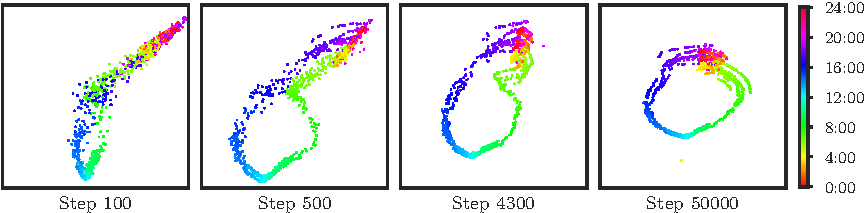
\includegraphics[height=.28\textheight]{z2_dynamic_latent_space}\\
    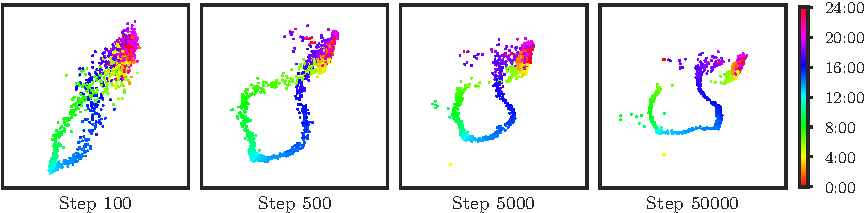
\includegraphics[height=.28\textheight]{z2_dynamic_latent_space_failed}
    \caption{
      Evolution of $q_{\phi}(\vv{z}|\vv{x})$ of dataset \DATASETB{} during training.
      \structure{Above}: a successful training (final F-score 0.871). \structure{Below}: a pathological training, converges to a sub-optimal equilibrium (final F-score 0.826).
    }
  \end{figure}
\end{frame}



%%%%%%%%%%%%%%%%%%%%%%%%%%%%%%%%%%%%%%%%%%%%%%%%%%%%%%%%%%%%%%%%%%%%%%%%%%%%%%%
% end input file: ./src/analysis.tex
%%%%%%%%%%%%%%%%%%%%%%%%%%%%%%%%%%%%%%%%%%%%%%%%%%%%%%%%%%%%%%%%%%%%%%%%%%%%%%%

%%%%%%%%%%%%%%%%%%%%%%%%%%%%%%%%%%%%%%%%%%%%%%%%%%%%%%%%%%%%%%%%%%%%%%%%%%%%%%%
% begin input file: ./src/conclusion.tex
%%%%%%%%%%%%%%%%%%%%%%%%%%%%%%%%%%%%%%%%%%%%%%%%%%%%%%%%%%%%%%%%%%%%%%%%%%%%%%%
\section{Conclusion}

%%%
\begin{frame}{Conclusion}
  Our unsupervised anomaly detection algorithm \DONUT{} for seasonal KPIs, based on VAE, greatly outperforms state-of-art supervised and vanilla VAE anomaly detection algorithms.  The best F-scores range from 0.75 to 0.90 for the studied KPIs.
  The key factors of \DONUT{} to be successful are:
  \begin{itemize}\setlength\itemsep{.2em}
    \item \structure{Dimension Reduction}: forces \DONUT{} to focus on the overall shape of normal patterns, and gain the ability of resisting abnormal points.
    \item \structure{M-ELBO, Missing Data Injection and MCMC Imputation}: further improves \DONUT{}'s ability to resist abnormal points.
  \end{itemize}
  
  Furthermore, we made the \emphasis{KDE Interpretation}, which provides a new perspective of VAE-based KPI anomaly detection.  All of the above factors can be verified by such interpretation.  The KDE Interpretation potentially has more theoretical value in the further development of deep generative models for KPI anomaly detection.\vspace{1em}
  
  \structure{\DONUT{} source code published at}: \url{https://github.com/korepwx/donut}.
\end{frame}

%%%
\begin{frame}{Thank you}
  \centering
  Q \& A
\end{frame}


%%%%%%%%%%%%%%%%%%%%%%%%%%%%%%%%%%%%%%%%%%%%%%%%%%%%%%%%%%%%%%%%%%%%%%%%%%%%%%%
% end input file: ./src/conclusion.tex
%%%%%%%%%%%%%%%%%%%%%%%%%%%%%%%%%%%%%%%%%%%%%%%%%%%%%%%%%%%%%%%%%%%%%%%%%%%%%%%


% Citation here
\begin{frame}[allowframebreaks] %allow to expand references to multiple frames (slides)
  \frametitle{References}
  \bibliographystyle{apa}
  \bibliography{references} %bibtex file name without .bib extension
\end{frame}

\end{document}
